% !TeX spellcheck = es_ANY
\documentclass[12pt,aspectratio=169]{beamer}
\setbeamercovered{transparent}

\usetheme{Madrid}
%\usetheme{Frankfurt}

\useinnertheme{circles}

\usepackage[utf8]{inputenc}
\usepackage[spanish,es-nodecimaldot]{babel}
\usepackage{amsmath}
\usepackage{mathtools}
\usepackage{amsfonts}
\usepackage{amssymb}
\usepackage{amsbsy}
%\usepackage{enumitem}
\usepackage{graphicx}
\usepackage[outdir=./figures/vect/]{epstopdf}
\usepackage{beamerfoils} % para usar \LogoOff
\usepackage{hyperref}% http://ctan.org/pkg/hyperref

\author[Luis M. Gato Díaz]{\small{Luis M. Gato D\'iaz\\ \href{mailto:lmiguelgato@comunidad.unam.mx}{lmiguelgato@comunidad.unam.mx}}} 

\institute[] % (optional, but mostly needed)
{	
	\tiny{Maestría en Ingeniería Eléctrica,	UNAM}
	
	\tiny{Posgrado de Procesamiento Digital de Señales}
}

%\date[21 de Mayo de 2019]
\date[\today]
{\includegraphics[height = 15mm]{figures/ingenieriaLOGO}\\
\small{Proyecto Final - Procesamiento Digital de Audio\\Profesor: Dr. Caleb Rascón Estebané}}

\title[Procesamiento Digital de Audio]{Localización y separación de múltiples fuentes de voz \\usando un arreglo de micrófonos}
%\subtitle{Tesis de diploma en opción al título de Ing. en Telecomunicaciones y Electrónica}
%\logo{\includegraphics[height = 10mm]{logo-cujae}}

\subject{Procesamiento Digital de Audio}
%\setbeamercovered{transparent}
\setbeamertemplate{navigation symbols}{}

\AtBeginSection[]
{
	\begin{frame}<beamer>{Sumario}
		\tableofcontents[currentsection,currentsubsection]
	\end{frame}
}

%\begin{document}
%	\maketitle
%	
%	\begin{frame}
%		\frametitle{}
%	\end{frame}
%\end{document}

\begin{document}
	
	\begin{frame}
		\titlepage
	\end{frame}
	
		\LogoOff
	
	\begin{frame}{Sumario}
		\tableofcontents %[pausesections]
		% You might wish to add the option [pausesections]
	\end{frame}
	

	
	\section{Descripción del problema}
	
	\begin{frame}{Descripción del problema}
		% - A title should summarize the slide in an understandable fashion
		%   for anyone how does not follow everything on the slide itself.
		\begin{figure}[h]
			\includegraphics[width=0.55\linewidth]{figures/array1.png}
		\end{figure}
	\hspace{7mm}\textbf{Tarea No. 1: Estimar la dirección en donde se localizan las fuentes de voz.}
	\end{frame}
	
	\begin{frame}{Descripción del problema}
		% - A title should summarize the slide in an understandable fashion
		%   for anyone how does not follow everything on the slide itself.
		\hspace{10mm}
		\begin{minipage}{60mm}
			\begin{figure}[h]
				\centering
				\includegraphics[width=0.95\linewidth]{figures/System}
			\end{figure}
		\end{minipage}
		\hspace{1mm}
		\begin{minipage}{70mm}
			\textbf{Requerimientos:}
			\begin{itemize}
				\item<1-| alert@1> Separación a ciegas: tanto las fuentes de voz como el proceso de mezclado son desconocidos.
				\pause
				\item<2-| alert@2> Únicamente se dispone de las grabaciones asociadas a cada elemento del arreglo.
				\pause
				\item<3-| alert@3> Maximizar la relación señal a interferencia.
				\pause
				\item<4-| alert@4> Presencia de niveles de ruido y de reverberación moderados.
				\pause
				\item<5-| alert@5-> Reducido costo computacional.
			\end{itemize}
		\end{minipage}
	
	\vspace{1mm}
	\hspace{7mm}\onslide<1->\textbf{Tarea No. 2: Separar las distintas fuentes de voz presentes en la mezcla.}
	\end{frame}
	
	\section{Modelo geométrico de propagación}
	
	\begin{frame}{Modelo geométrico de propagación}
		\begin{block}{Ecuación de onda en medios homogéneos y no dispersivos:}
		\begin{equation}
		\frac{\partial^2 E(t, \mathbf{r})}{\partial x^2} + \frac{\partial^2 E(t, \mathbf{r})}{\partial y^2} + \frac{\partial^2 E(t, \mathbf{r})}{\partial z^2} = \frac{1}{c^2}\frac{\partial^2 E(t, \mathbf{r})}{\partial t^2}
		\label{EcOnda}
		\end{equation}
		\end{block}
		\textbf{Si la fuente es un emisor puntual:}
		\begin{equation}
		\frac{\partial^2 \{r E(t, \mathbf{r})\}}{\partial r^2} = \frac{1}{c^2}\frac{\partial^2 \{r E(t, \mathbf{r})\}}{\partial t^2}
		\label{EcOnda1}	
		\end{equation}
		\textbf{Solución de la ecuación de onda:}		
		\begin{equation}
		E(t, \mathbf{r}) = s(t-r/c)
		\label{EcOndaSol1}
		\end{equation}
		\textbf{Ejemplo:} señales complejas de banda estrecha
		$E(t, \mathbf{r}) = A e^{j(\omega t - \mathbf{k}\cdot\mathbf{r})} = A e^{j\omega t} e^{-j\mathbf{k}\cdot\mathbf{r}}$
	\end{frame}	
	
	\begin{frame}{Modelo geométrico de propagación}
		\textbf{Detección tridimensional de una fuente:}
		\begin{equation}
		\mathbf{x}(t) = 
		\begin{bmatrix}
		x_1(t) \\
		x_2(t) \\
		\vdots \\
		x_M(t)
		\end{bmatrix}
		=
		\begin{bmatrix}
		e^{-j\mathbf{k}(\theta, \phi)\cdot \mathbf{r}_1} \\
		e^{-j\mathbf{k}(\theta, \phi)\cdot \mathbf{r}_2} \\
		\vdots \\
		e^{-j\mathbf{k}(\theta, \phi)\cdot \mathbf{r}_M}
		\end{bmatrix} 
		s(t) = \mathbf{a}(\theta, \phi) s(t)
		\label{EcArray}
		\end{equation}
		
		\vspace{10mm}
		\textbf{Detección bidimensional de varias fuentes contaminadas con ruido:}
		\begin{equation}
		\mathbf{x}(t) = 
		\mathbf{A}(\pmb{\theta}) \mathbf{s}(t) + \mathbf{w}(t)
		\label{EcArray1}
		\end{equation}
	\end{frame}
	
	\begin{frame}{Modelo geométrico de propagación}
		\textbf{Modelo de campo lejano:}
		\begin{figure}[h]
			\centering
			\includegraphics[width=0.7\linewidth]{figures/array2.png}
		\end{figure}
	\end{frame}
	
	\begin{frame}{Modelo geométrico de propagación}
		\textbf{Modelo de campo lejano:}
		\begin{figure}[h]
			\centering
			\includegraphics[width=0.7\linewidth]{figures/array3.png}
		\end{figure}
	\end{frame}
	
	\section{Estimación de las direcciones de arribo}
	
	\begin{frame}{Estimación de las direcciones de arribo}
	\textbf{Vector de correlación cruzada con transformada de fase:}
	\begin{equation}
	r_{pq}[k] = \frac{1}{N} \sum\limits_{m = 0}^{N-1} \frac{X_p[m]X_q^*[m]}{|X_p[m]| |X_q[m]|} e^{j2\pi km/N}~~~~~~~~\mathrm{para~}k_{\mathrm{min}}\le k\le k_{\mathrm{max}}
	\end{equation}
%	\begin{equation}
%	\mathrm{CCV}[k] = \frac{\sum_{i} (x_i - m_x) (y_{i-k} - m_y)}{\sqrt{\sum_i (x_i - m_x)^2} \sqrt{\sum_i (y_{i-k} - m_y)^2}}~~~~~~~~\mathrm{para~}k_{\mathrm{min}}\le k\le k_{\mathrm{max}}
%	\end{equation}
	\begin{figure}[h]
		\centering
		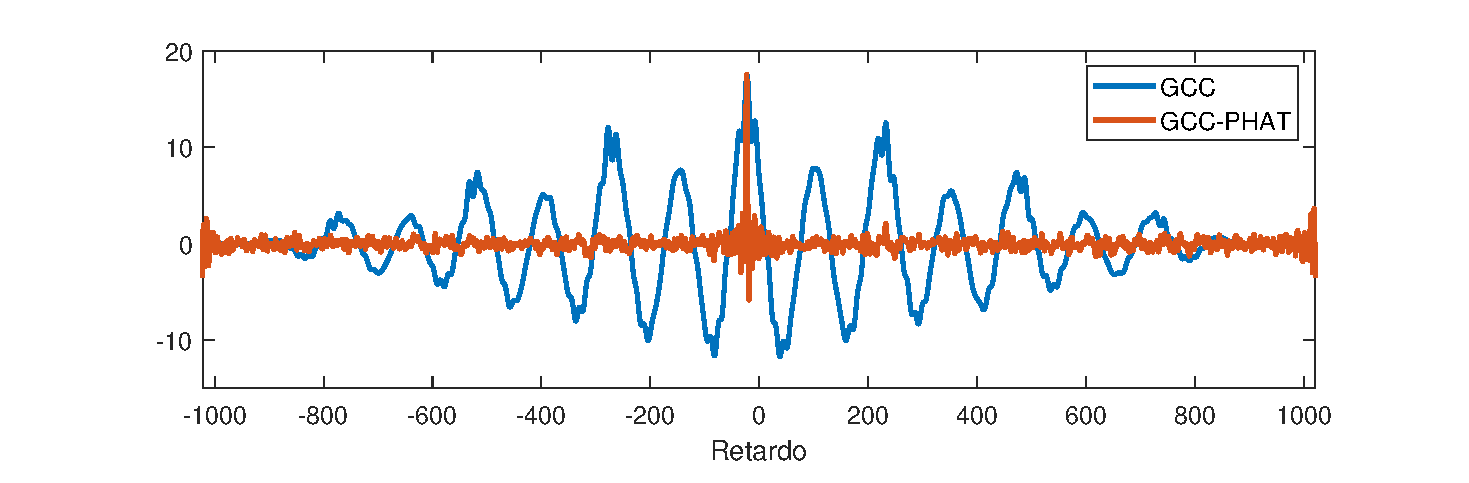
\includegraphics[width=\linewidth]{figures/GCCvsGCCphat}
	\end{figure}
	\end{frame}
	
	\begin{frame}{Estimación de las direcciones de arribo}
		\textbf{Vector de correlación cruzada con transformada de fase:}
		\begin{equation}
		r_{pq}[k] = \frac{1}{N} \sum\limits_{m = 0}^{N-1} \frac{X_p[m]X_q^*[m]}{|X_p[m]| |X_q[m]|} e^{j2\pi km/N}~~~~~~~~\mathrm{para~}k_{\mathrm{min}}\le k\le k_{\mathrm{max}}
		\end{equation}
		\begin{figure}[h]
			\centering
			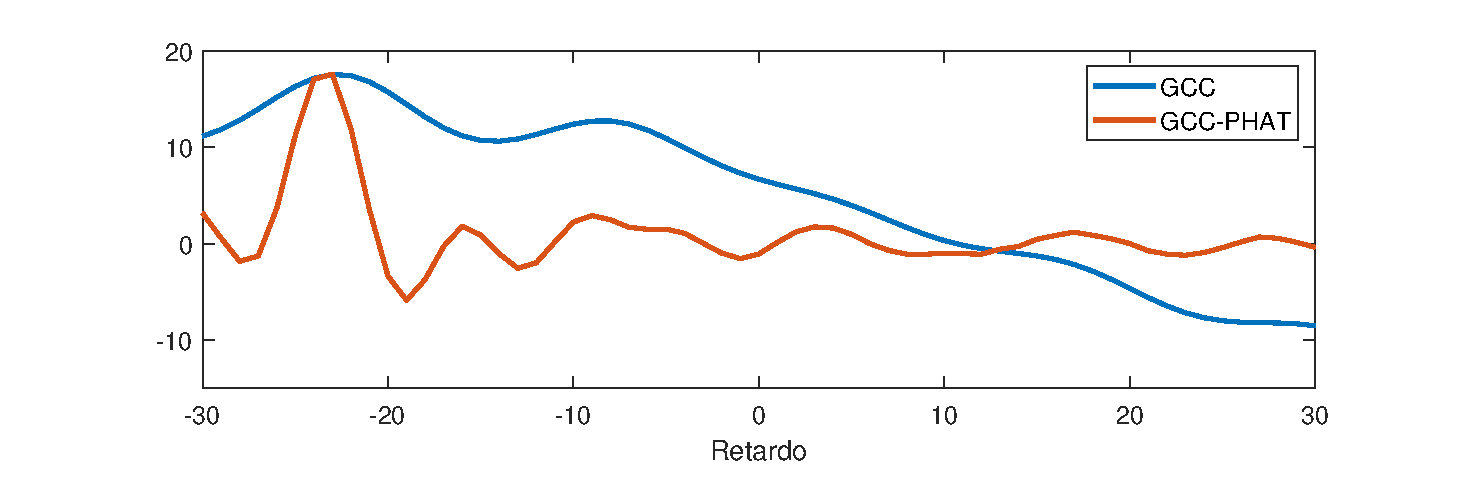
\includegraphics[width=\linewidth]{figures/zoomGCCvsGCCphat}
		\end{figure}
	\end{frame}

	\begin{frame}{Estimación de las direcciones de arribo}
	\textbf{Ajustes al método de correlación:}	
	\begin{itemize}
		\item<1-> Se usó un umbral para descartar niveles bajos de correlación: $r_{pq}[k]_{max} > \gamma_0$
		\pause
		\item<2-> Luego se incluyó un umbral adaptativo: \\
		a$)~\gamma_n = 0.9 \frac{(n-1)\gamma_{n-1} + max\{r_{pq}[k]_{max}\}}{n}$ ~~~~~~
		b$)~\gamma_n = 0.9 \frac{(n-1)\gamma_{n-1} + \overline{r_{pq}[k]_{max}}}{n}$
	\end{itemize}
	\begin{figure}[h]
		\centering
		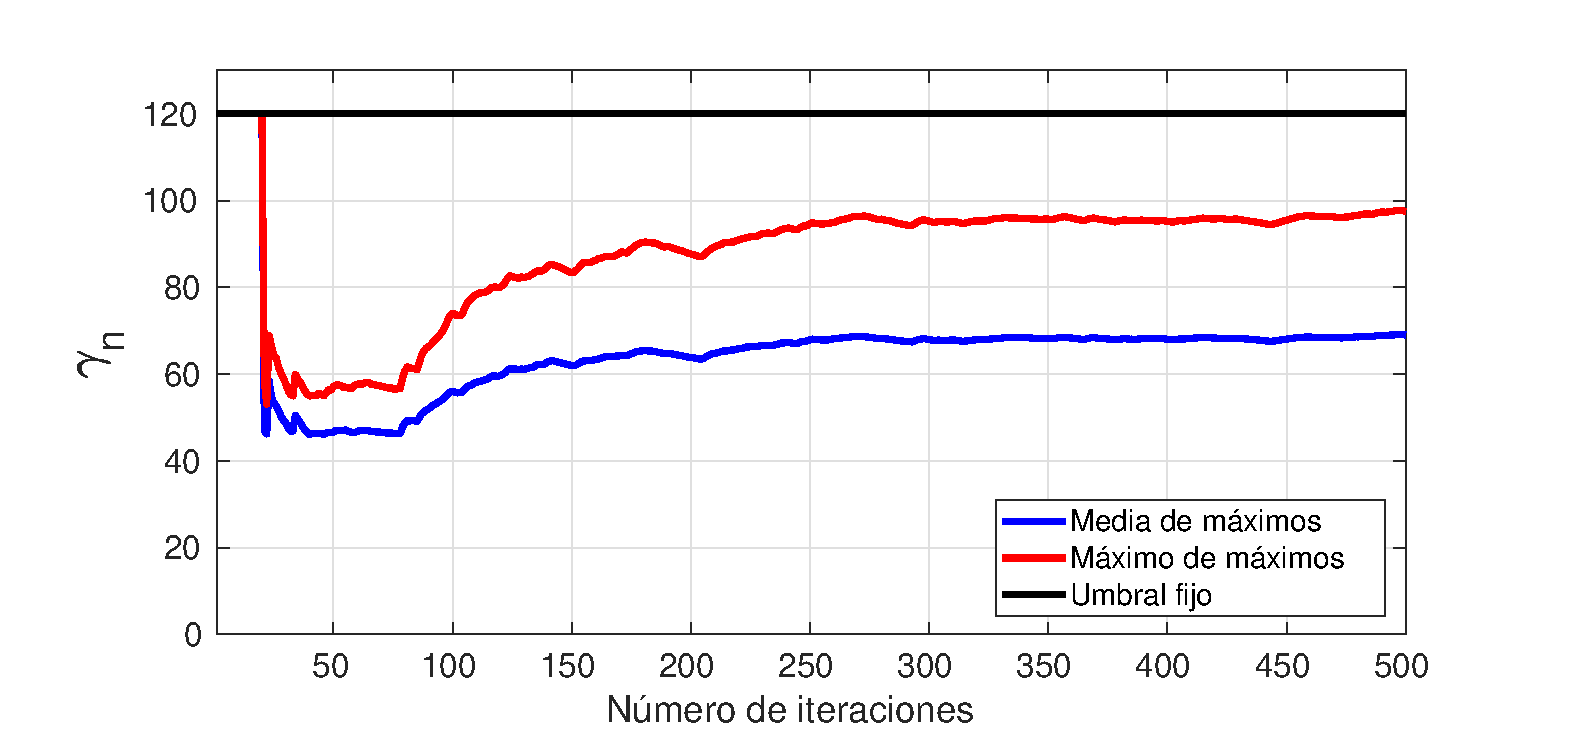
\includegraphics[width=0.65\linewidth]{figures/threshold.eps}
	\end{figure}
	\end{frame}
	
	\begin{frame}{Estimación de las direcciones de arribo}
		\textbf{Se estima, para cada par de micrófonos la dirección de arribo:}
		\begin{equation}
			\theta_{12} = \frac{\mathrm{sen}^{-1}(c \Delta t_{12})}{d}~~~~~\theta_{23} = \frac{\mathrm{sen}^{-1}(c \Delta t_{23})}{d}~~~~~\theta_{31} = \frac{\mathrm{sen}^{-1}(c \Delta t_{31})}{d}
		\end{equation}		
		\hspace{5mm}
		\begin{minipage}{70mm}
			\begin{figure}[h]
				\centering
				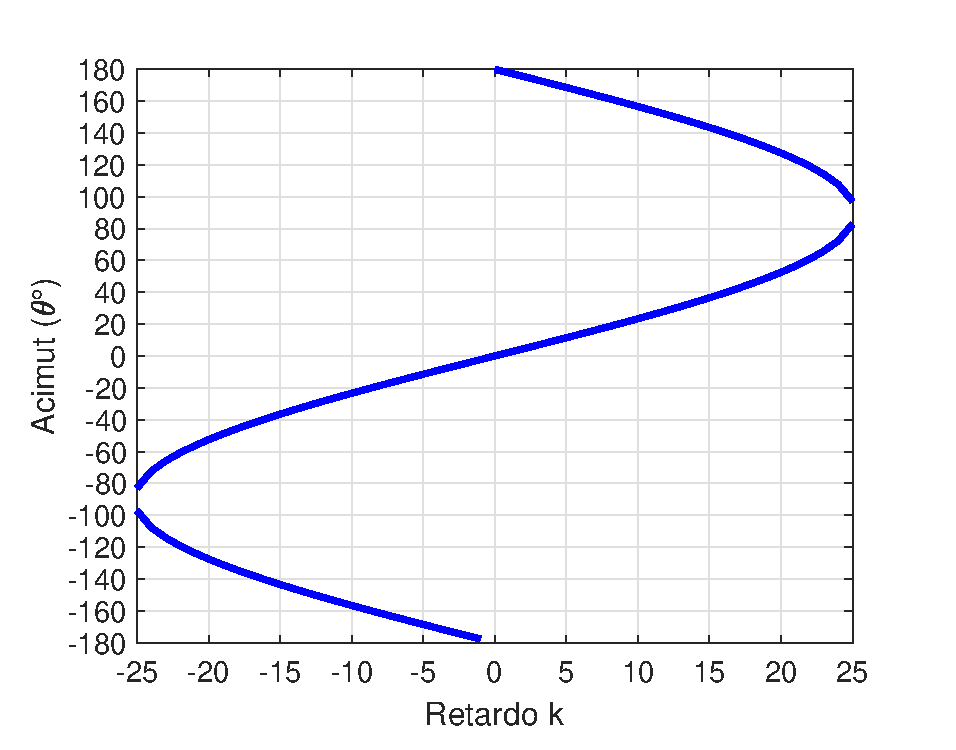
\includegraphics[width=0.9\linewidth]{figures/DOAvsDelay}
			\end{figure}
		\end{minipage}
		\hspace{10mm}
		\begin{minipage}{50mm}
			\begin{figure}[h]
				\centering
				\includegraphics[width=\linewidth]{figures/reference}
			\end{figure}
		\end{minipage}
		
	\end{frame}
	
	\begin{frame}{Estimación de las direcciones de arribo}
		\textbf{Se determina si existe redundancia en las direcciones de arribo:}
		\begin{equation}
		\left[\theta_{12}; \theta'_{12}\right]~~~~~\left[\theta_{23}; \theta'_{23}\right]+120^{\mathrm{o}}~~~~~\left[\theta_{31}; \theta'_{31}\right]-120^{\mathrm{o}}
		\end{equation}		
		\hspace{5mm}
		\begin{minipage}{70mm}
			\begin{figure}[h]
				\centering
				\includegraphics[width=\linewidth]{figures/redundancia}
			\end{figure}
		\end{minipage}
	\hspace{5mm}
		\begin{minipage}{60mm}
			Existen $2^3$ pares distintos de ángulos, de los cuales se pueden obtener 2 o hasta 3 pares que \textit{apuntan} aproximadamente a la misma dirección.
			\vspace{5mm}	
		
			\pause
			
			Se estableció un umbral de coherencia: $\Delta \theta < 30^{\mathrm{o}}$
		\end{minipage}
	\end{frame}

	\begin{frame}{Estimación de las direcciones de arribo}
	\textbf{Fuentes de voz que no coinciden por breves segmentos de tiempo ...}
	\begin{figure}[h]
		\centering
		\includegraphics[width=0.5\linewidth]{figures/nonoverlap}
	\end{figure}
	\end{frame}
	
	\begin{frame}{Estimación de las direcciones de arribo}
		\textbf{... proporcionan conjuntos distinguibles de direcciones de arribo, asociados a las distintas fuentes presentes:}
		
		\begin{figure}[h]
			\centering
			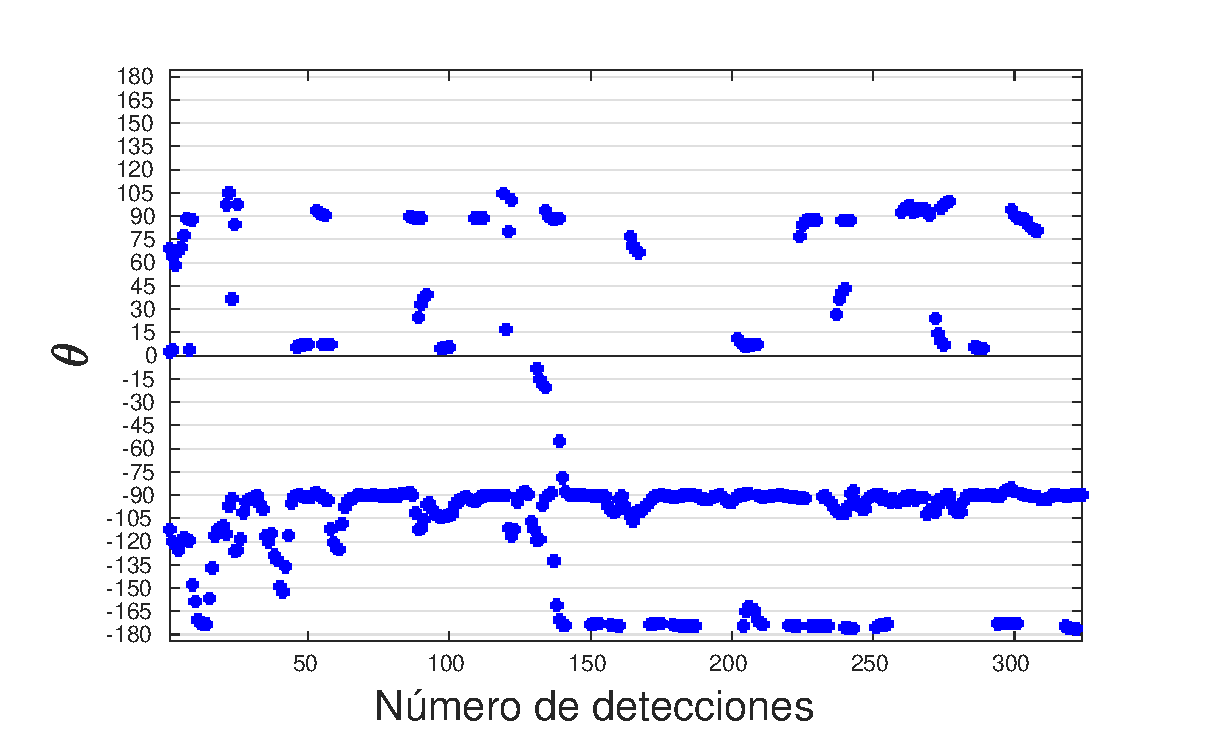
\includegraphics[width=0.65\linewidth]{figures/plot4uncolor}
		\end{figure}
	\end{frame}
	\begin{frame}{Estimación de las direcciones de arribo}
		\textbf{Se usó el algoritmo de clasificación $k$-\textit{means} para distinguir las distintas fuentes, suponiendo que no hay dos fuentes en una misma dirección.}
		
		\begin{figure}[h]
			\centering
			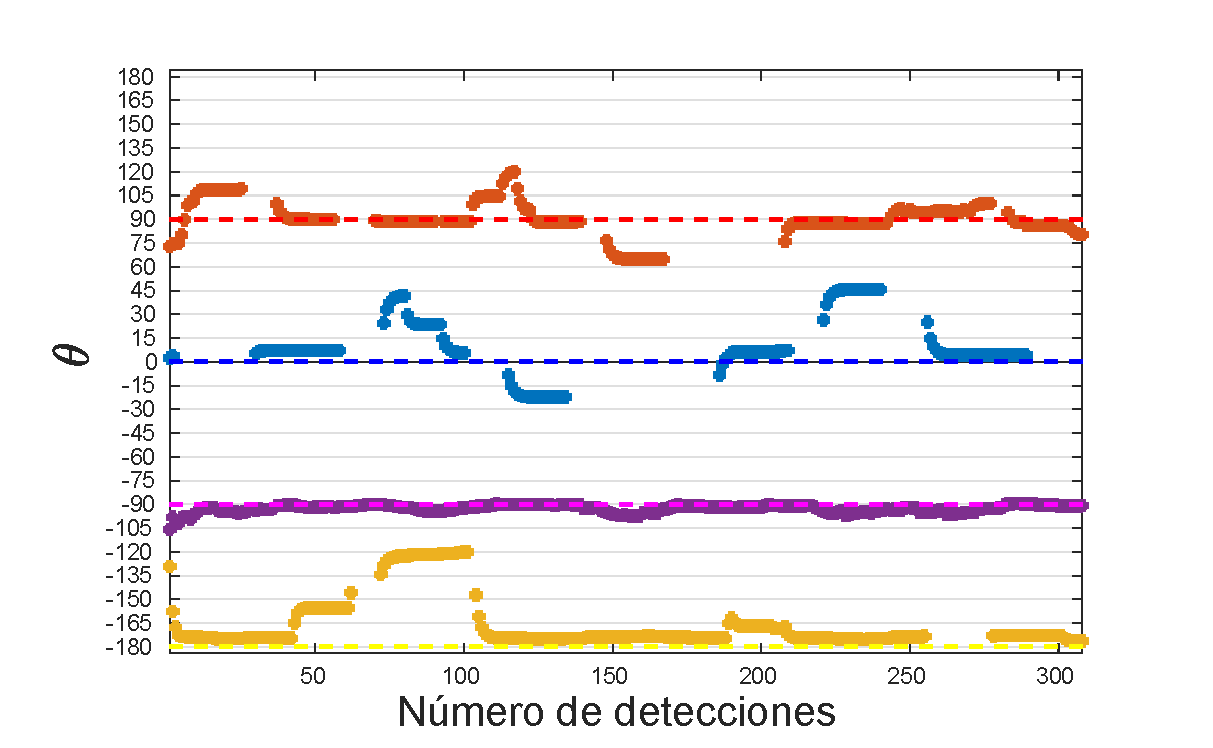
\includegraphics[width=0.65\linewidth]{figures/plot4colornomean}
		\end{figure}
	\end{frame}
	
	\begin{frame}{Estimación de las direcciones de arribo}
		\textbf{Se aplicó a los centroides de $k$-means un filtro de media móvil y un umbral de desviación respecto a la media.}
		
		\begin{figure}[h]
			\centering
			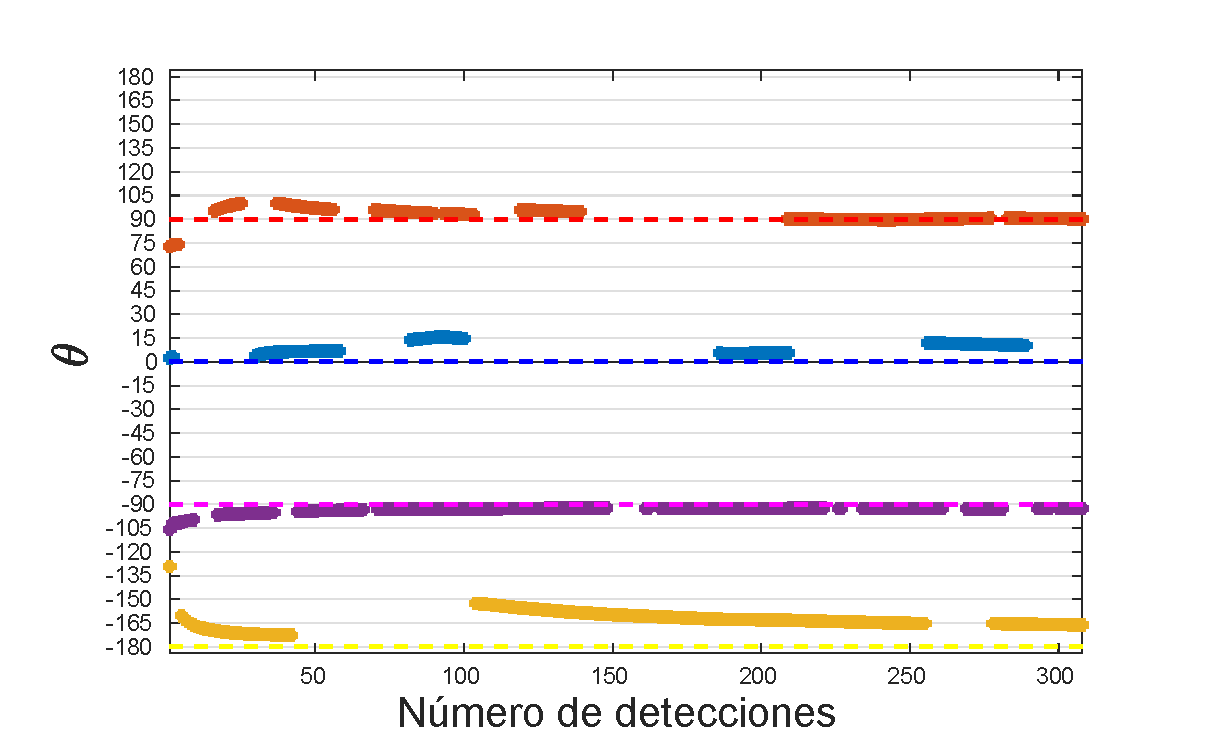
\includegraphics[width=0.65\linewidth]{figures/plot4color}
		\end{figure}
	\end{frame}
	
%	\begin{frame}{Estimación de las direcciones de arribo}
%		\textbf{Se aplicó a los centroides de $k$-means un filtro de media móvil y un umbral de desviación respecto a la media.}
%		
%		\begin{figure}[h]
%			\centering
%			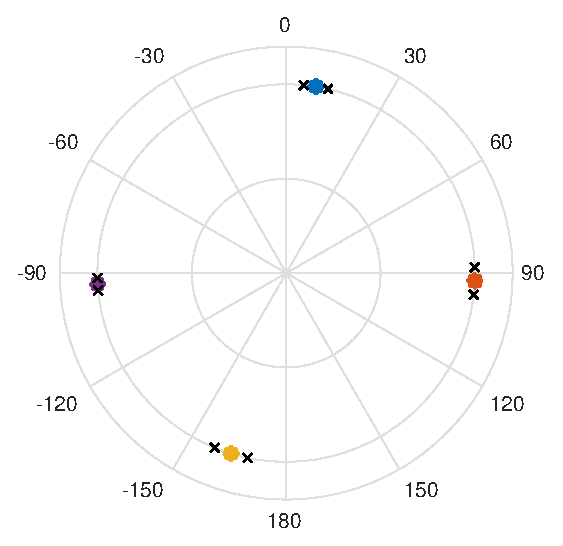
\includegraphics[width=0.4\linewidth]{figures/polar4color}
%		\end{figure}
%	\end{frame}
	
%	\begin{frame}{Estimación de las direcciones de arribo}
%		\textbf{Estas modificaciones permiten también extender el método a fuentes móviles:}
%		
%		\hspace{20mm}
%		\begin{minipage} {105mm}
%			\begin{figure}[h]
%				\centering
%				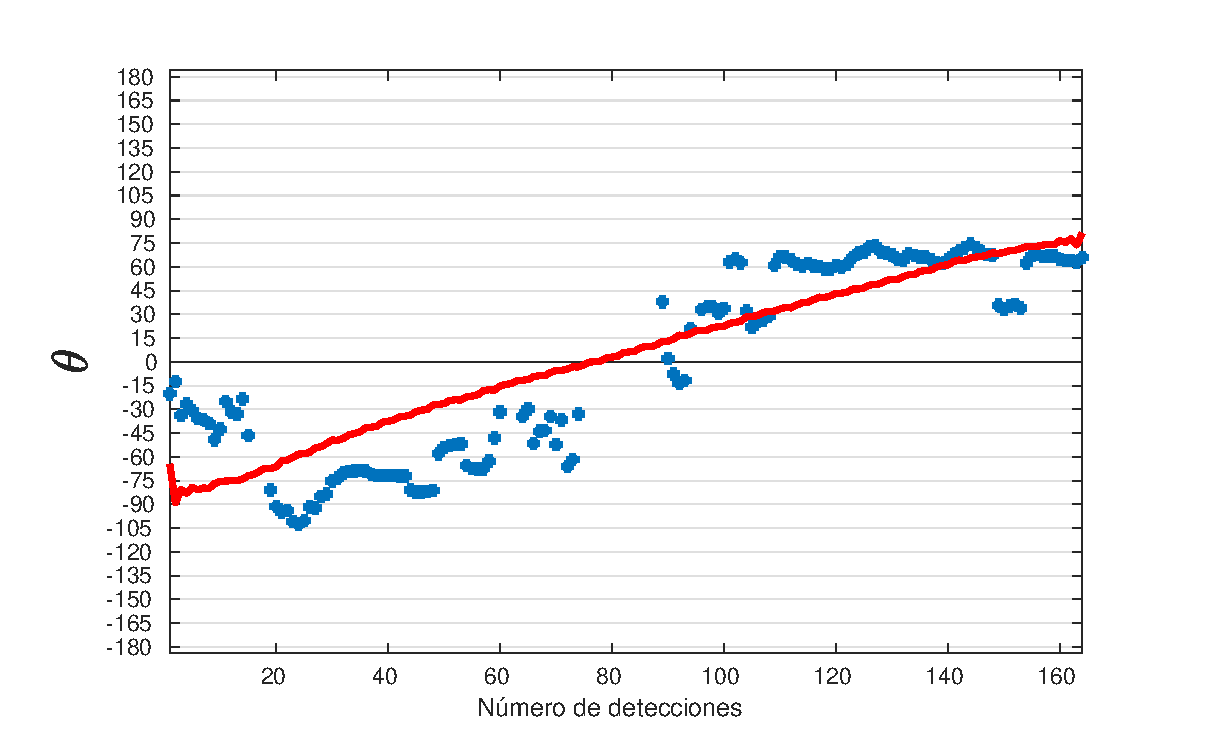
\includegraphics[width=\linewidth]{figures/moving1nomean}
%			\end{figure}
%		\end{minipage}\\
%		\hspace{130mm}\textbf{antes ...}
%	\end{frame}
%	
%	\begin{frame}{Estimación de las direcciones de arribo}
%		\textbf{Estas modificaciones permiten también extender el método a fuentes móviles:}
%		
%		\hspace{20mm}
%		\begin{minipage} {105mm}
%			\begin{figure}[h]
%				\centering
%				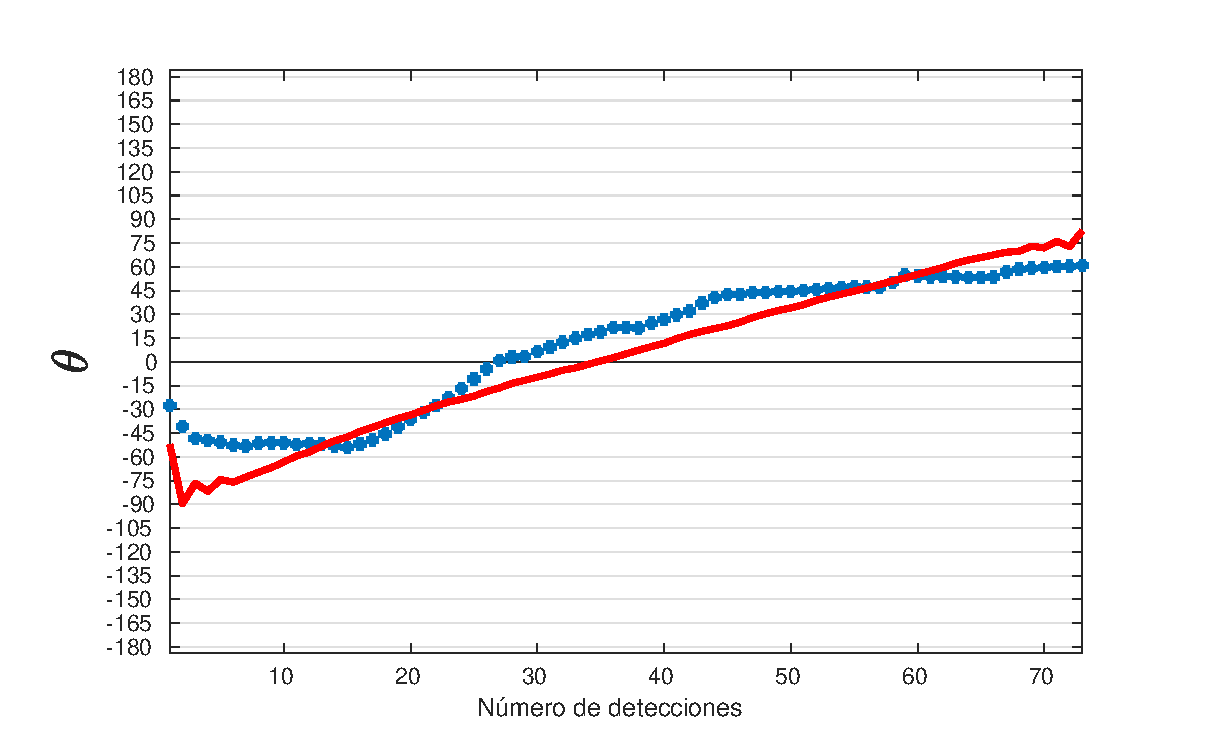
\includegraphics[width=0.98\linewidth]{figures/moving130kmean10degrees}
%			\end{figure}
%		\end{minipage}\\
%		\hspace{130mm}\textbf{... después.}
%	\end{frame}
	
	\section{Separación de las fuentes de voz}
	
	\begin{frame}{Separación de las fuentes de voz}
		\textbf{Formador de haz de retardos y sumas:}\\	
		\vspace{5mm}
		\begin{figure}[h]
			\centering
			\includegraphics[width=0.7\linewidth]{figures/steer}
		\end{figure}
	\end{frame}
	
	\begin{frame}{Separación de las fuentes de voz}
		\textbf{Formador de haz de retardos y sumas:}\\	
		\vspace{5mm}
		\begin{figure}[h]
			\centering
			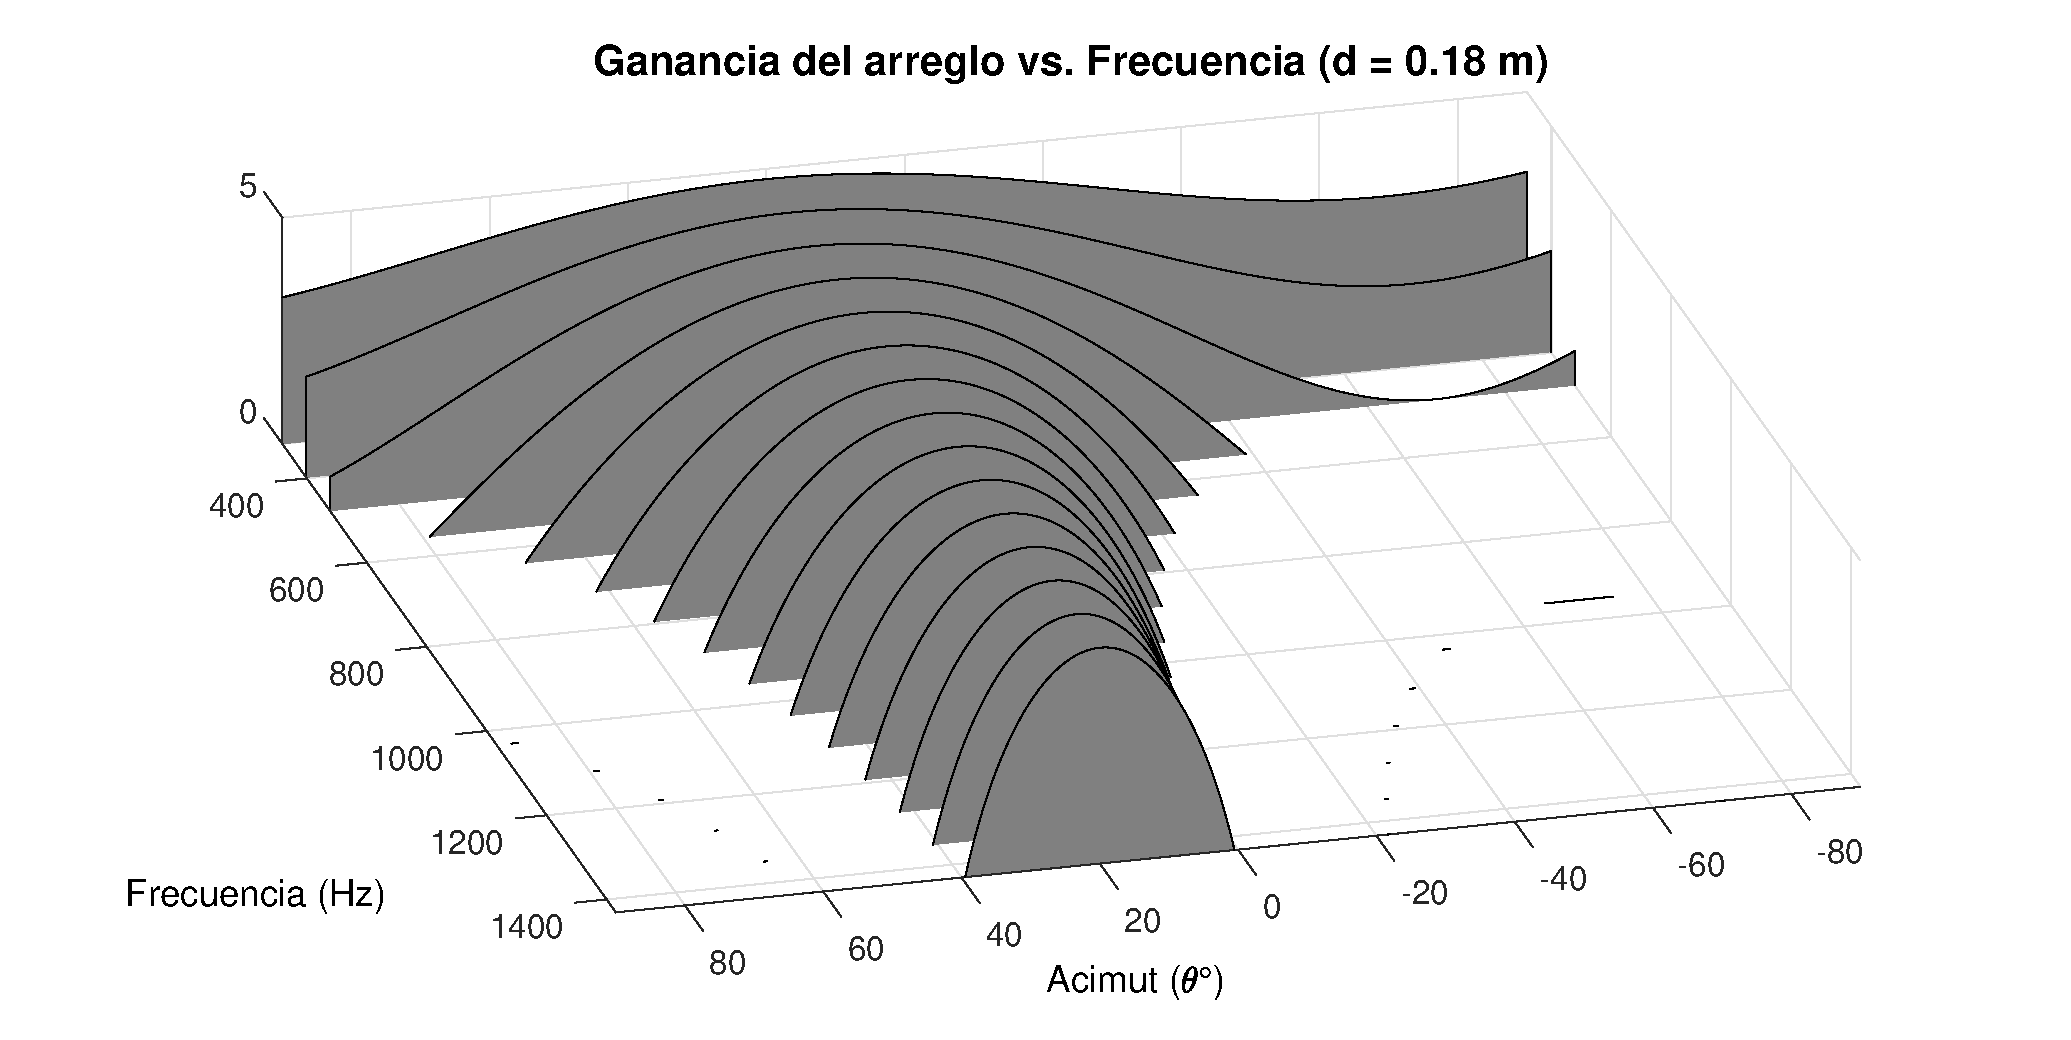
\includegraphics[width=0.8\linewidth]{figures/patternvsfreq}
		\end{figure}
	\end{frame}
	
	\begin{frame}{Separación de las fuentes de voz}
		\textbf{Se aplican los retardos operando en el dominio de la frecuencia, sobre dos buffers solapados de 4 ventanas de datos (overlap-add):}\\		
		\vspace{5mm}
		\begin{figure}[h]
			\centering
			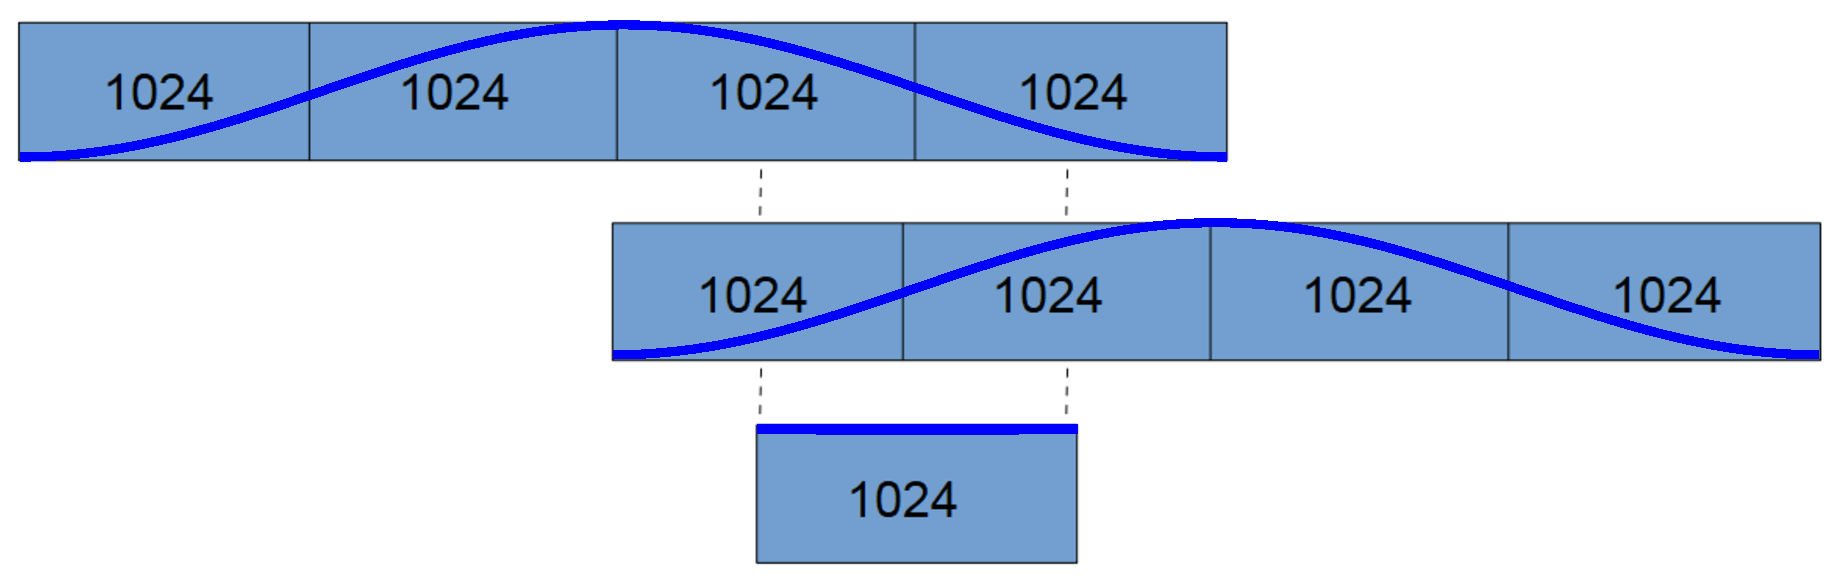
\includegraphics[width=0.8\linewidth]{figures/Buffers.eps}
		\end{figure}
	\end{frame}
	
	\section{Resultados}
	
%	\begin{frame}{Resultados}
%		\begin{minipage}{70mm}
%			\textbf{Cámara anecoica: $\pmb{\theta} = [0, 90, 180]$}
%			\begin{figure}[h]
%				\centering
%				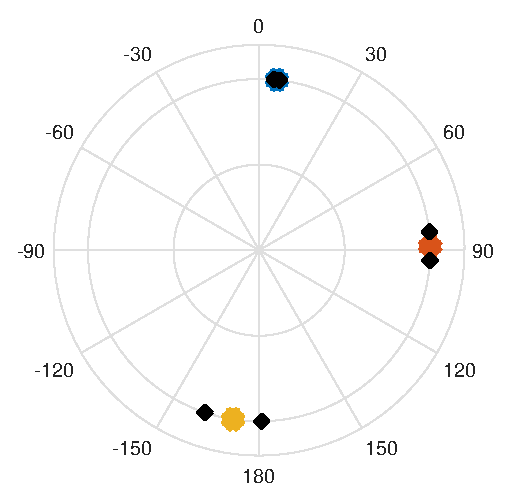
\includegraphics[width=0.9\linewidth]{figures/3Clean.eps}
%			\end{figure}
%		\end{minipage}
%		\begin{minipage}{70mm}
%			\hspace{10mm}\textbf{Oficina: $\pmb{\theta} = [0, 90, 180]$}
%			\begin{figure}[h]
%				\centering
%				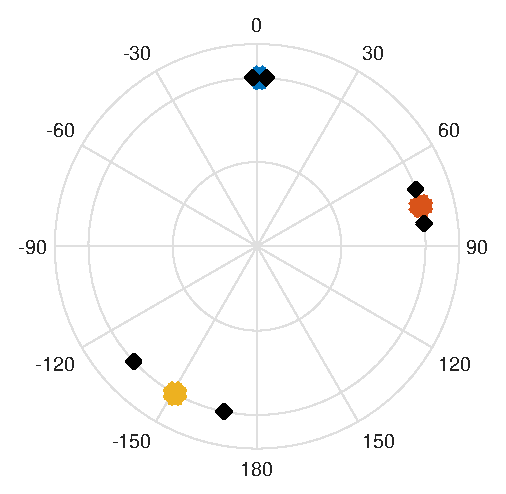
\includegraphics[width=0.9\linewidth]{figures/3Noisy.eps}
%			\end{figure}
%		\end{minipage}
%	\end{frame}
	
	\begin{frame}{Resultados}
		\begin{minipage}{70mm}
			\textbf{Cámara anecoica: $\pmb{\theta} = [-90, 0, 90, 180]$}
			\begin{figure}[h]
				\centering
				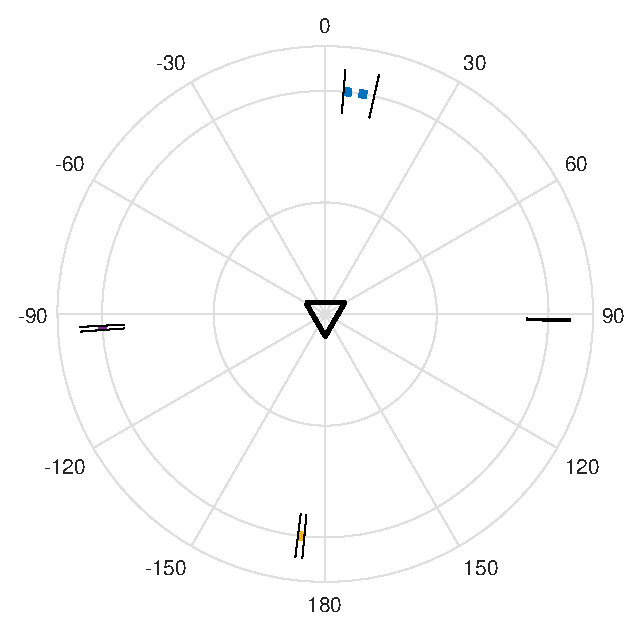
\includegraphics[width=0.9\linewidth]{figures/4Clean.eps}
			\end{figure}
		\end{minipage}
		\begin{minipage}{70mm}
			\hspace{10mm}\textbf{Oficina: $\pmb{\theta} = [-90, 0, 90, 180]$}
			\begin{figure}[h]
				\centering
				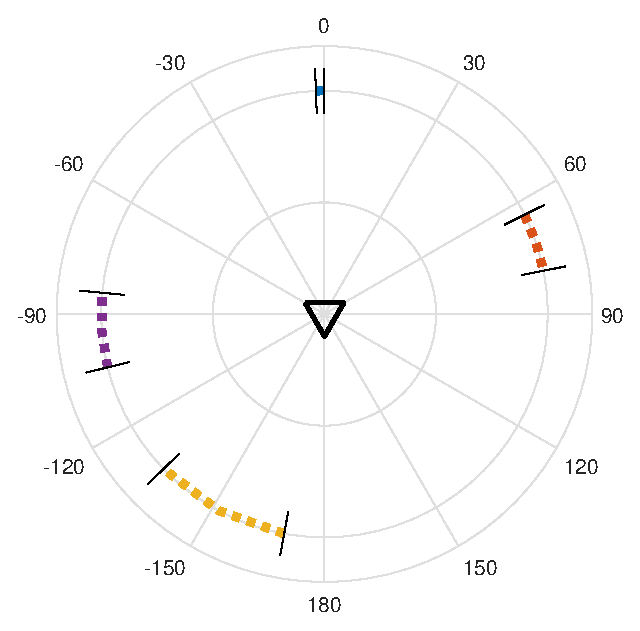
\includegraphics[width=0.9\linewidth]{figures/4Noisy.eps}
			\end{figure}
		\end{minipage}
	\end{frame}
	
	\begin{frame}{Resultados preliminares}
		\textbf{Fuentes en movimiento:}
		
		\hspace{20mm}
		\begin{minipage} {105mm}
			\begin{figure}[h]
				\centering
				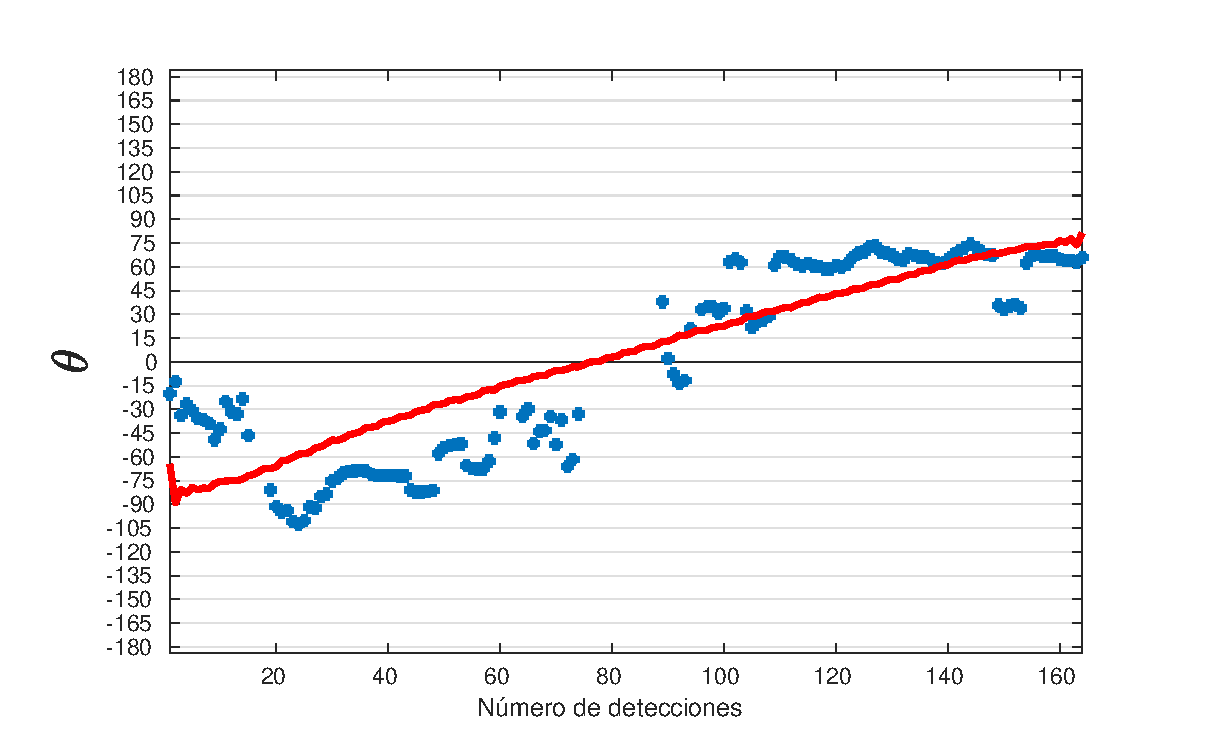
\includegraphics[width=\linewidth]{figures/moving1nomean}
			\end{figure}
		\end{minipage}\\
		\hspace{130mm}\textbf{antes ...}
	\end{frame}
	
	\begin{frame}{Resultados preliminares}
		\textbf{Fuentes en movimiento:}
		
		\hspace{20mm}
		\begin{minipage} {105mm}
			\begin{figure}[h]
				\centering
				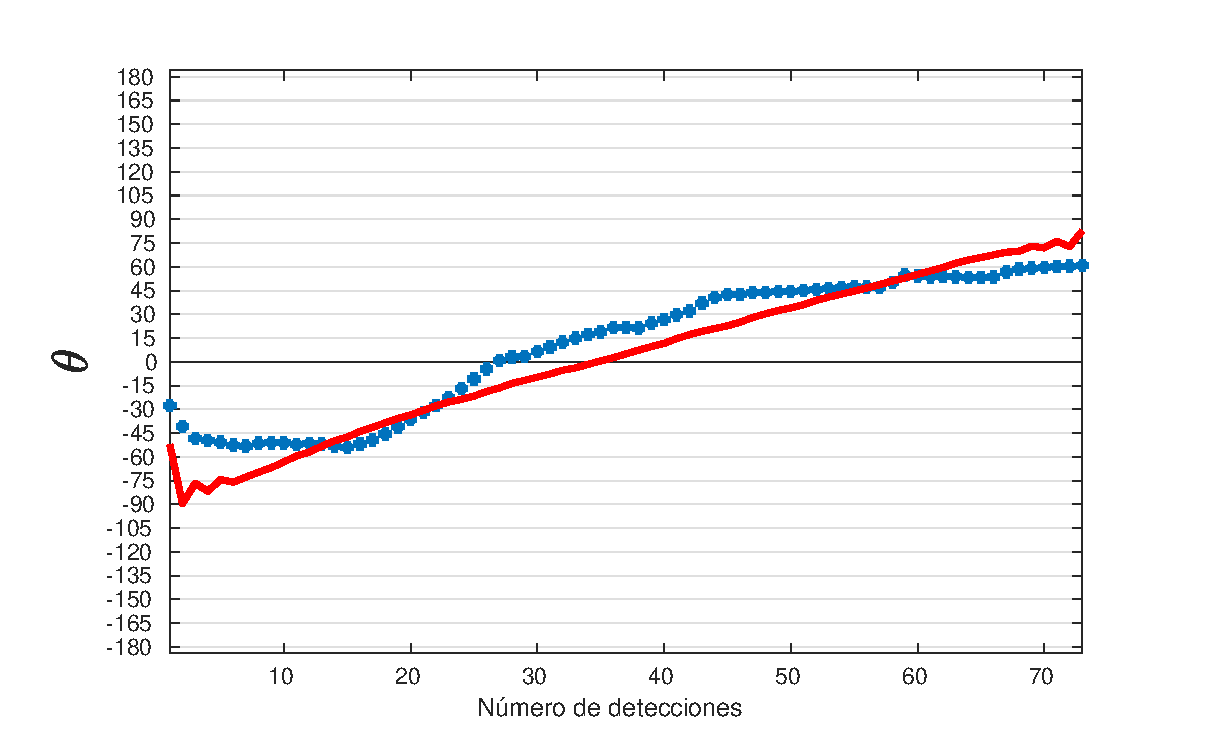
\includegraphics[width=0.99\linewidth]{figures/moving130kmean10degrees}
			\end{figure}
		\end{minipage}\\
		\hspace{130mm}\textbf{... después.}
	\end{frame}
	
	\begin{frame}{Resultados}
		\textbf{Se usó la librería BSS\_EVAL\footnote{E. Vincent, R. Gribonval and C. Févotte, \textit{Performance measurement in blind audio source separation}, IEEE Trans. Audio, Speech and Language Processing, 14(4), pp 1462-1469, 2006.} para evaluar el desempeño del formador de haz, y estos son algunos ejemplos de resultados obtenidos:}
		\begin{table}[H]
			\begin{center}
				\begin{tabular}{|c||c|c|}
					\hline Número & máx\{$\Delta$SIR\} con & máx\{$\Delta$SIR\} con \\ 
					de fuentes & el estimado de $\pmb{\theta}$ & conocimiento perfecto de $\pmb{\theta}$ \\ 
					\hline \hline 
					2 & 3.1 & 8.0  \\
					\hline 									 			
					3 & 3.5 & 9.1 \\
					\hline 									 			
					4 & 2.3 & 2.8  \\
					\hline 							
				\end{tabular}
			\end{center}
		\end{table}
		\vspace{-3mm}
		\pause
		\color{red} \textbf{En general, el desempeño del separador de las voces depende fuertemente del desempeño del localizador de las fuentes de voz.}
	\end{frame}
	
%	\begin{frame}{Resultados}
%		Función de costo $C_{ML}$ evaluada sobre la superficie $\{\theta_1,\theta_2\} \in \{-30^{\mathrm{o}}, 30^{\mathrm{o}}\}\times\{-30^{\mathrm{o}}, 30^{\mathrm{o}}\}$ para un escenario con dos fuentes localizadas en $\pmb{\theta} = [-10^{\mathrm{o}}~~18^{\mathrm{o}}]^T$ y $\sigma^2 = 0$.$02$.
%		\begin{figure}[h]
%			\centering
%			\includegraphics[width=0.52\linewidth]{figures/Fig3a.png}
%		\end{figure}
%	\end{frame}
%	
%	\begin{frame}{Resultados}
%		Función de costo $C_{B}$ evaluada sobre la superficie $\{\theta_1,\theta_2\} \in \{-30^{\mathrm{o}}, 30^{\mathrm{o}}\}\times\{-30^{\mathrm{o}}, 30^{\mathrm{o}}\}$ para un escenario con dos fuentes localizadas en $\pmb{\theta} = [-10^{\mathrm{o}}~~18^{\mathrm{o}}]^T$ y $\sigma^2 = 0$.$02$.
%		\begin{figure}[h]
%			\centering
%			\includegraphics[width=0.52\linewidth]{figures/Fig3.png}
%		\end{figure}
%	\end{frame}
	
%	\begin{frame}{Resultados}
%		Estimación de las direcciones de arribo de tres fuentes localizadas en $\pmb{\theta} = [3^{\mathrm{o}}~~8^{\mathrm{o}}~~15^{\mathrm{o}}]^T$.				
%		\begin{figure}[h]
%			\centering
%			\includegraphics[width=0.58\linewidth]{figures/Fig21.png}
%		\end{figure}
%	\end{frame}
%	
	
	
	
	
	\section{Conclusiones}
	
	\begin{frame}{Conclusiones}
		\begin{itemize}
			\item Se ha obtenido un método de \textbf{bajo costo computacional} que permite localizar \textbf{al menos 4} fuentes de voz de forma simultánea.		
			\vspace{0.1in}
			\pause
			\item Relativamente \textbf{buena precisión} ante ruido y reverberación moderados.			
			\vspace{0.1in}
			\pause
			\item El desempeño se \textbf{deteriora significativamente} cuando las fuentes están en movimiento.			
			\vspace{0.1in}
			\pause
			\item No requiere conocer exactamente el número de fuentes presentes, pero sí el \textbf{número máximo de fuentes} para la clasificación.
		\end{itemize}
	\end{frame}


%\logo{\includegraphics[height = 10mm]{logo-cujae}}
		
\begin{frame}

		\titlepage

	\end{frame}
	
\end{document}


